\chapter{Value-gradient Aware Model Learning}
\label{chap:vagram}

\begin{quote}
    This chapter is based on \longfullcite{voelcker2022value}.
\end{quote}

\newcommand{\revised}[1]{#1}
\section{Introduction}
\ac{mbrl} is a sample-efficient approach to obtain a policy for a given control problem. 
It solves the control optimization into two interleaved stages: model learning and policy learning or planning. 
In the \emph{model learning} stage, an approximate model of the environment is learned which is then utilized in the \emph{planning} stage to generate new experience without having to query the original environment. 
Often this process is repeated by continuously updating the model with new experience and replanning based on the updated model. 
\ac{mbrl} is an enticing paradigm for scenarios in which samples of the true environment are difficult or expensive to obtain, such as computationally intensive simulators, real-world robots, or environments involving humans, since the model can be used to generalize the policy to unseen regions of the state space. 
The approach has received a lot of attention and significant progress has been made in the field \parencite{dyna,deisenroth2011pilco,levine2013guided,hafner2020dream,moerland,schrittwieser2020mastering}.

One of the core problems of model-based policy learning methods, however, is that the accuracy of the model directly influences the quality of the learned policy or plan \parencite{schneider1997exploiting,kearns2002near,ross2012agnostic,talvitie2017self,luo2018algorithmic,mbpo}. 
Model errors tend to accumulate over time, and therefore long-term planning under approximate models can lead to suboptimal policies compared to the performance achievable with model-free approaches.
This is especially prevalent in settings with complex dynamics, such as robotic environments with discontinuities, which can be hard to model with common function approximation methods.
These model approximation errors are nearly impossible to avoid with current methods due to limits of function approximation in model and value learning algorithms, which cannot fully capture the full distribution over dynamics functions perfectly, and the use of finite datasets.

Hence, it is important that a model is accurate \textit{where it counts} for the planning procedure, by modelling dimensions and data points that have a higher impact on the planning.
But this objective is not captured in most current \ac{mbrl} methods, which generally use \ac{mle}-based losses to train a parametric model of the environment without involving information from the planning process.
The misalignment between the \emph{model learning} and \emph{planning} stages of \ac{mbrl} has received renewed interest and is now commonly termed the \textit{objective mismatch} of reinforcement learning~\parencite{lambert202objective}, but the problems has been investigated in earlier works \parencite{joseph2013reinforcement}.
Several recent papers have investigated the objective mismatch~\parencite{abachi2020policy,zhang2021learning,ayoub2020model,grimm2020value,grimm2021proper,nikishin2021control}, but currently theoretical investigation and understanding of possible approaches do not perform well when applied to complex deep learning based approaches~\parencite{lovatto2020decision} or the proposed approaches rely on heuristics which might not be applicable generally~\parencite{nair2020goal}.

\noindent \textbf{Summary of Contributions}. We present the \textit{Value-Gradient Weighted MOdel Learning}~(VaGraM) which rescales the mean squared error loss function with gradient information from the current value function estimate.
We demonstrate the advantage of the VaGraM loss over previous approaches via the analysis of the optimization behavior of the Value-Aware Model Learning framework \parencite{vaml, itervaml} and form two hypotheses for the lack of empirical performance gain despite theoretical intuition: (a) the theory does not account for the optimization trajectory induced by the loss function and (b) it also does not address how to counter problems that arise when the state-space is yet insufficiently explored in early stages of the model training.
Our experiments show, qualitatively and quantitatively, that the VaGraM loss impacts the resulting state and value prediction accuracy, and that it solves the optimization problems of previously published approaches.
Beyond pedagogical domains, we show that VaGraM performs on par with a current state-of-the art \ac{mbrl} algorithms in more complex continuous control domains, while improving robustness to irrelevant dimensions in the state-space and smaller model sizes.



\section{Value-Gradient Weighted Model Learning (VaGraM)}
\label{sec:vagram:method}

One of the main drawbacks of model-based reinforcement learning is the fact that model errors propagate and compound when the model is used for planning \parencite{schneider1997exploiting,kearns2002near,talvitie2017self}.
As discussed in \autoref{chap:background:objective}, one attempt at addressing the objective mismatched is the IterVAML loss \parencite{itervaml}
\begin{align}
    &\mathcal{L}_V(\hat{p}, p, \mu) = \int \mu(\state,a) \bigg|\overbrace{\int p(\state'|\state,a)V(\state')\mathrm{d}\state'}^{\text{environment value estimate}}  - \overbrace{\int \hat{p}(\state'|\state,a) V(\state') \mathrm{d}\state'}^{\text{model value estimate}}\bigg|^2 \mathrm{d} (\state,a)
\end{align}

\textcite{itervaml} present error bounds for both steps of the iteration, but did not test the algorithm to ascertain whether the presented error bounds are sufficient to guarantee \revised{a strong algorithm in practice}. 
As we discuss now, IterVAML provides an intuitive fix to the model-mismatch problem, yet faces two key issues which lead to empirical ineffectiveness.  
These phenomena are investigated and verified in detail in \autoref{sec:vagram:experiments}.

% To address these, we propose Value-Gradient Weighted MOdel Learning (VaGraM), a loss which is value-aware and has stable optimization behavior even in challenging domains with function approximation.

\paragraph{Value function evaluation outside of the empirical state-action distribution} IterVAML suffers when randomly initialized models predict next states that are far away from the current data distribution or if the optimization procedure leads the model's prediction outside of the covered state space. 
Since the value function has only been trained on the current data distribution, it will not have meaningful values at points outside of its training set.
Nonetheless, these points can still achieve small value prediction errors if, due to the optimization process, the value function outside the training distribution happens to have the same value at the model prediction as at the environment sample.
We therefore require that our value-aware loss function should not directly depend on the value function at the model prediction, since these might be potentially meaningless.

\revised{\paragraph{Suboptimal local minima} %We also observe that the algorithm often moves to local minima in the state space, which incur large losses once the value function is updated.
Since the model can converge to a solution that is far away from the environment sample if the values are equal, we find that the model-based value prediction often performs poorly after updating the value function.
We expect that the updated model loss forces the model prediction to a new solution, but due to the non-convex nature of the VAML loss, the model can get stuck or even diverge.
This is especially prevalent when the previous minimum is situated outside of the empirically covered state space.
A stable value-aware loss function should therefore have only one minimum in the state space that lies within the empirical state distribution.\footnote{\revised{The full loss function will likely still admit additional local minima due to the non-linear nature of the model itself, but the global optimum should coincide with the true model and the loss function should be convex in the state space.}}}

\subsection{Approximating a value-aware loss with the value function gradient}
From our insights, we obtain two criteria: a stable loss should not depend on the value function at states not captured in the dataset, and it should not admit local minima beyond an \ac{mle} solution.
To derive a loss function that fulfils these requirements, we start from the assumption that the difference between the model prediction and the environment next states $\state'$ are small.
This is implicitly required by many \ac{mbrl} approaches, since an MLE model cannot be used to estimate the next state's value otherwise. 
\revised{We also assume that the model has small transition noise, akin to the model assumptions underlying MSE regression, otherwise the difference between a model sample and the next state sample might be large.}
Under this assumption, the IterVAML loss can be approximated by a Taylor expansion of the value function, where we denote the expansion of $V$ around a reference point $\state'$ as $\hat{V}_{\state'}$ and obtain $\hat{V}_{\state'}(\state) \approx V(\state') + (\nabla_\state V(\state)|_{\state'})^\intercal (\state - \state')$.
Using this expansion at the next state sample $\state'_i \in \mathcal{D}$ collected from the environment for each tuple independently instead of the original value function, the VAML error can be stated as:
% \vspace{-10pt}
\begin{align}
    \hat{\mathcal{L}}_{\hat{V}}=&\sum_{\{\state_i,a_i,\state'_i\}\in\mathcal{D}}{\left(V(\state'_i) - \int \hP_\theta(\state'|\state_i,a_i) (V(\state'_i) + (\nabla_\state V(\state)|_{\state'_i})^\intercal (\state' - \state'_i)) \mathrm{d}\state'\right)^2}\\
    =&\sum_{\{\state_i,a_i,\state'_i\}\in\mathcal{D}} {\left(\int \hP_\theta(\state'|\state_i,a_i) \left((\nabla_\state V(\state)|_{\state'_i})^\intercal(\state' - \state'_i) \right) \mathrm{d}\state'\right)^2}
\end{align}

This objective function crucially does not depend on the value function \revised{at unknown state samples, all $\state'_i$ are in the dataset the value function is trained on}, which solves the first of our major problems with the VAML paradigm.

We can simplify the objective above even further if we restrict ourselves to deterministic models of the form $\hat{\state}'_i = f_\theta(\state,a)$.
Since VAML requires the expectation of the value function under the model and the environment to be equal, we can exchange the probabilistic model with a deterministic one as long as we assume that the mean value function under the true environment is close to the empirical estimate of the value function from a single sample.
We explore the prerequisites and consequences of this assumption further in \autoref{chap:cvaml}.
The model loss can then be expressed as:
% \vspace{-5pt}
\begin{align}
    \sum_i {\left((\nabla_\state V(\state)|_{\state'_i})^\intercal (f_\theta(\state_i,a_i) - \state'_i) \right)^2} \label{eq:vagram:taylor_vaml}
\end{align}

We can see that the objective is similar to a mean squared error regression with a vector that defines the local geometry of the objective function. This vector can be interpreted as a measure of sensitivity of the value function at each data point and dimension. In regions where the value function changes significantly, the regression pushes the model to be very accurate. 

\subsection{Bound between Value-Aware Model Learning and VaGraM}
\label{app:taylor_bound}

The error in Taylor approximation $\mathcal{R}(V, s', f_\theta(s,a))$ is bounded by $\frac{M}{2}||s' - f_\theta(s,a)||^2$ with M dependent on the Hessian of the value function. Plugging this into the VAML loss and assuming worst case approximation errors, we obtain an upper bound on the VAML error:

\begin{align*}
    &\E_{s',s,a \sim D}\left[\left(V\left(f_\theta(s,a) \right) - V(s_0')\right)^2\right] \\
    = &\E_{s',s,a \sim D}\left[\left((\nabla_s V(s)|_{s'})^\intercal (f_\theta(s,a) - s') + \mathcal{R}(V, s',f_\theta(s,a))\right)^2\right]\\
    \leq &\E_{s',s,a \sim D}\left[\left(\left|(\nabla_s V(s)|_{s'})^\intercal (f_\theta(s,a) - s')\right| + \left|\mathcal{R}(V, s_0', f_\theta(s,a))\right|\right)^2\right]\\
    \leq &\E_{s',s,a \sim D}\left[{\left(\left|(\nabla_s V(s)|_{s'})^\intercal (f_\theta(s,a) - s')\right| + \frac{M}{2}||s' - f_\theta(s,a)||^2\right)^2}\right]\\
    \leq &2\cdot\E_{s',s,a \sim D}\left[{\left((\nabla_s V(s)|_{s'})^\intercal (f_\theta(s,a) - s')\right)^2}\right] + 2\cdot\E_{s',s,a \sim D}\left[\frac{M^2}{4}||s' - f_\theta(s,a)||^4\right]
\end{align*}

Our experiments show that if we treat $M$ like a tuneable hyperparameter, optimization difficulties appear.
We conjecture that in practice, this problem is caused by the difficulty of estimating the spectrum of the Hessian.
We find that most often, either the first or the second loss component will dominate when choosing values heuristically.
However, without bounding the second term, we are faced with the issue of spurious local optima which we address now.


\subsection{Preventing spurious local minima}
\begin{figure}[!t]
\centering
    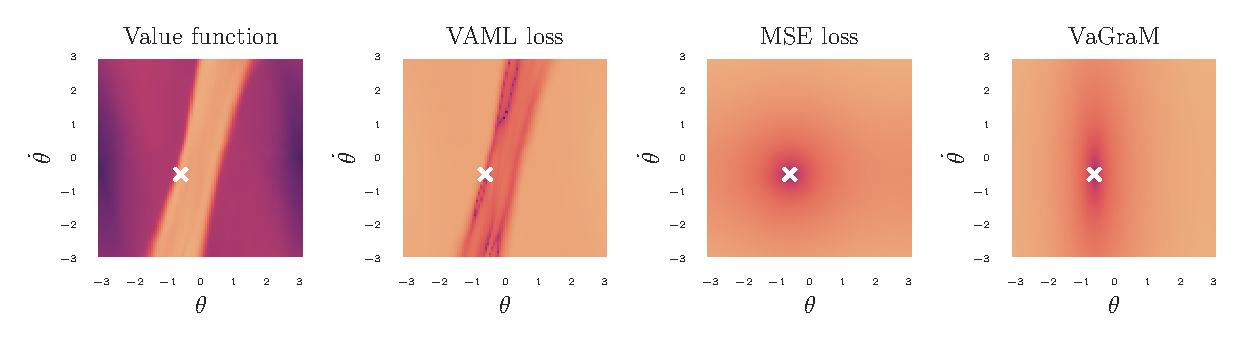
\includegraphics[clip, trim=0.cm 0.5cm 0.cm 0.45cm, width=\textwidth]{figures/vagram/all_losses.pdf}
    \caption{\revised{Visualization of discussed loss function with regards to a reference point marked with the white cross and the corresponding value function on the Pendulum environment. For the value function, darker color indicates a lower value. In the loss figures, darker color indicates how large the loss is if the model predicts $(\theta, \dot{\theta})$ instead of the reference sample marked in white. The VAML loss has a complex non-linear shape in the state space that follows iso-lines of the value function, while MSE and VaGraM are centered around the sample. For VaGraM, the rescaling of the MSE in the direction of high gradient along the $\theta$ axis is visible. Due to \autoref{eq:vagram:upper_bound}, the scaling is aligned with the axis of the coordinate system and not rotated to fit the value function closer.}}
    \label{fig:vagram:all_losses}
\end{figure}


The formulation above retains one problem, \autoref{eq:vagram:taylor_vaml} does not constrain the solution for each $(\state,a,\state')$ tuple sufficiently.
For each $(\state,a,\state')$ tuple, the loss function only requires that the difference between the model and environment sample be orthogonal to the gradient of the value function, which describes a hyperplane of solutions.
These predictions can lie arbitrarily far away from the environment sample, which breaks the assumption underlying the Taylor approximation that the model prediction is within a small region of the expanded state point.
This can be made more clear by looking at the loss for a single datapoint
\begin{align}
    &\min_\theta \left((\nabla_\state V(\state)|_{\state'})^\intercal f_\theta(\state,a) \right) ^2\\
    =&\min_\theta \left(\sum_{n=0}^{\text{dim}(\states)} (\nabla_\state V(\state)|_{\state'})_n \cdot f_\theta(\state,a)_n\right)^2
\end{align}

Assuming that $f$ is flexible and can predict any next state $\state'$, the optimal solution is obtained from an undetermined linear system of equations
\begin{align}
    \sum_{n=0}^{\text{dim}(\states)} (\nabla_s V(s)|_{s'})_n \cdot f_\theta(s,a)_n = 0
\end{align}

This system admits far more solutions than either the corresponding IterVAML loss or a mean squared error, and many of them will achieve arbitrary large value prediction errors.
In fact, the equation describes a hyperplane of minimal solutions consisting of every weight vector that is orthogonal to the gradient of the value function at the reference sample, with $\text{dim}(\mathcal{S}) - 1$ free variables.
Therefore we need to enforce the closeness of the model prediction and the environment sample, since the Taylor approximation is only approximately valid in a close ball around the reference sample.

One way to achieve this closeness is by adding the second order Taylor term, which results in an additional MSE loss term.
However, we did not achieve good performance when testing out this version, as it is difficult to compute the Hessian in higher-dimensional state spaces 
Therefore, we approached the solution to this problem as outlined below.

\subsection{Bounding the first-order Taylor loss}

To prevent these suboptimal solutions and achieve our second design goal, we consider an upper bound on the value-gradient loss by applying the Cauchy Schwartz inequality $\left(\sum_{i=1}^n x_i \right) ^2 \leq n \sum x_i^2$ to change the square of the sum with a sum of squares.
We denote the diagonal matrix with vector $a$ on the diagonal as $\text{diag}(a)$ and refer to the dimensionality of the state space as $\text{dim}(\mathcal{S})$ and rephrase the sum as a vector-matrix multiplication:
% \vspace{-5pt}
\begin{align}
    &\sum_{\{s_i,a_i,s'_i\}\in\mathcal{D}} {\left((\nabla_s V(s)|_{s'_i})^\intercal(f_\theta(s_i,a_i) - s'_i) \right)^2}\\
    \leq {\text{dim}(\mathcal{S})} &\sum_{\{s_i,a_i,s'_i\}\in\mathcal{D}}\left((f_\theta(s_i,a_i) - s'_i)^\intercal\text{diag}(\nabla_s V(s)|_{s'_i})^2(f_\theta(s_i,a_i) - s'_i) \right) \label{eq:vagram:upper_bound}.
\end{align}

This reformulation is equivalent to a mean squared error loss function with a per-sample-dimension diagonal scaling matrix.
Because the scaling matrix is positive semi-definite by design, each summand in the loss is a quadratic function with a single solution as long as the derivative of the value function does not become zero in any component.
Therefore this upper bound assures our second requirement: the loss function does not admit spurious local minima.\footnote{We note that state dimensions are ignored for points in which components of the value function become zero, potentially leading to spurious minima as before solutions, but in practice this rarely happens for more than a few points.}

To give an intuitive insight into all the discussed loss functions, we visualized each one for a pedagogical environment, the Pendulum stabilization task.
The resulting loss curves can be seen in \autoref{fig:vagram:all_losses}.
The VAML loss has a complicated shape that depends on the exact values of the value function while both MSE and our proposal have a paraboloid shape.
Compared to MSE, our proposed loss function is rescaled to account for the larger gradient of the value function in the $\theta$ axis.

\section{Experiment: Model learning in low-dimensional problem}
\label{sec:vagram:experiments}
% \begin{figure}[t]
% \centering
%     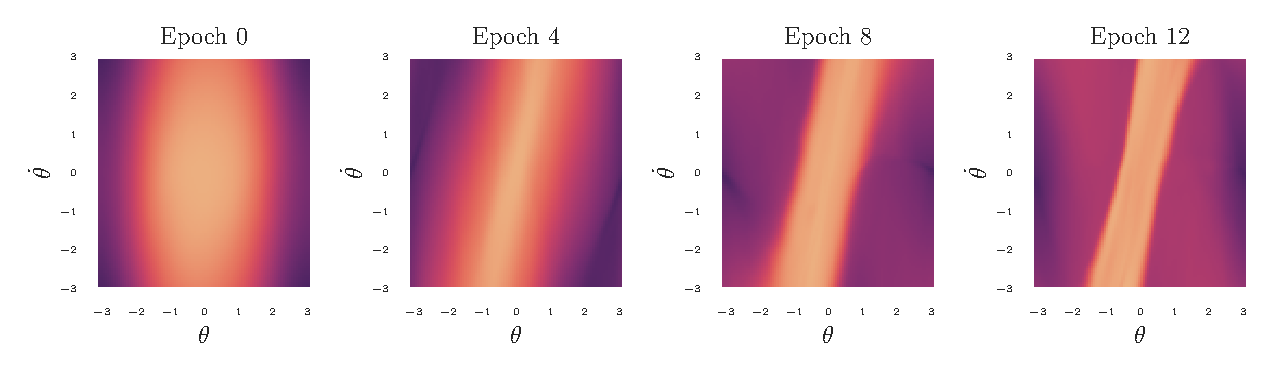
\includegraphics[width=1.\textwidth]{figures/vagram/value_functions.png}
%     \caption{Empirical value functions learned by SAC over several training epochs. Darker color corresponds to smaller value. While the learned value function is not exactly equivalent to the known correct solution for the problem (compare \parencite{lutter}) the approximation highlights the shape of the value function and the sharp edges at the points of destabilization.}
%     \label{fig:vagramvf_pendulum}
% \end{figure}

\begin{figure}[t]
\begin{center}
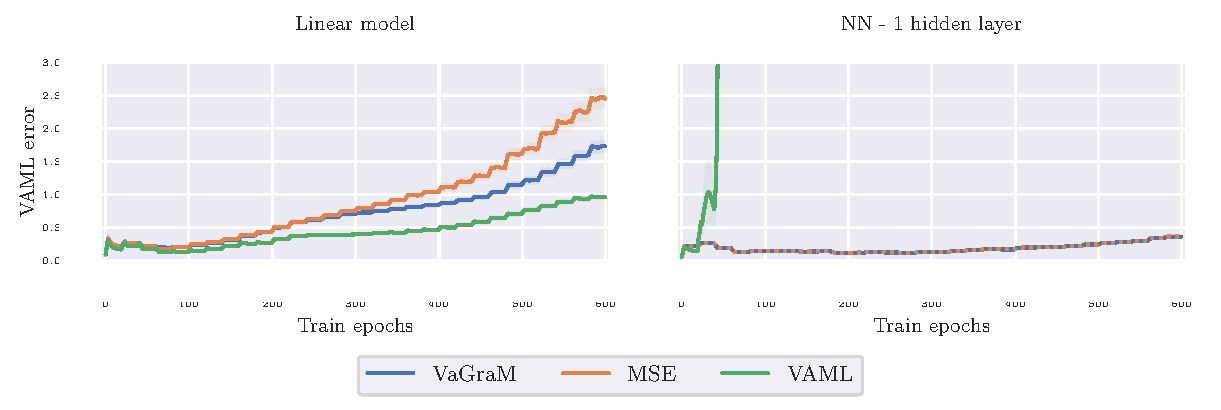
\includegraphics[width=\linewidth]{figures/vagram/pendulum_joint.pdf}
\end{center}
\caption{\textbf{Evolution of the VAML loss over changing value functions on the Pendulum domain}. Lines denote the mean and shaded areas show standard error over 8 model initialization and data set samples per model. In the linear setting, VAML achieves the lowest VAML error, while VaGraM is able to significantly outperform MSE. In the NN setting, VAML diverges rapidly, \revised{while VaGraM and MSE converge to approximately the same solution.}}
\label{fig:vagram:iterated_pendulum_training}
\end{figure}

We compare the performance of VaGraM, with both MSE and VAML on a pedagogical environment with a small state space and smooth dynamics to gain qualitative insight into the loss surfaces. 
We use the Pendulum environment, a canonical control problem in which an under-actuated pendulum must be swung and stabilized to an upright position.
We use the implementation provided by \cite{brockman2016openai}.
%The state of the problem is $(\sin(\theta), \cos(\theta), \dot{\theta})^\intercal$ and the action space $\ddot\theta$ is bounded between $[-1, 1]$.
%To visualize the value function fully, we transform the Cartesian representation into polar coordinates. 
To learn the policy and its value function, we use the SAC algorithm \parencite{sac}.
The original IterVAML analysis assumed that the value function was obtained using approximate value iteration (AVI) \parencite{gordon1995stable,ernst2005tree,farahmand2010error}. We use SAC instead of a full AVI for stability in large scale experiments and discuss a proper extension of the VAML loss to SAC in \autoref{app:vagram:vaml_sac}. We find that the difference in loss is negligible and therefore use SAC together with VAML throughout our experiments.
More information on the implementation and hyperparameters of all of our experiments can be found in \autoref{app:vagram:implementation}. 

To simplify the setup of the evaluation, we decided to investigate the model losses without model-based value function learning.
This allows us to focus solely on the loss functions, without taking into account the inter-dependency between model and value function updates.
Instead of the model-based loop, we used the SAC algorithm in a model-free setup to estimate the value function.
We saved the intermediate value functions after each epoch of training, corresponding to 200 environment steps, and optimized the models using stochastic gradient descent on the respective loss function, updating the value function used for the loss every 1000 model training steps.
As the MLE loss, we used the mean squared error which assumes a Gaussian model with fixed variance.

To compare the optimization, we used two architectures, a linear regression without feature transformations and a neural network with a single hidden layer and 16 neurons.
We obtained a dataset of states sampled uniformly over the whole state space and used the environment transition function to compute ground truth next state samples.
Finally, we evaluated each models VAML error with regards to the current value function on a held out dataset and plotted the results in \autoref{fig:vagram:iterated_pendulum_training}.

\paragraph{Dependency on untrained value function estimates.}
The first cause for lacking empirical performance with VAML that we discussed in \autoref{sec:vagram:method} was that the algorithm can predict successor states with incorrect value function as they lie outside of the data distribution.

In our experiment we find that a linear regression model remains stable under all three loss functions, VaGraM, MSE and VAML.
But when using a flexible function approximation, the VAML loss converges in the first iteration with the given value function, but then rapidly diverges once the value function is updated.
When investigating the mean squared error of the VAML solution, we find that the model finds a stable minimum of the VAML loss outside of the reachable state space of the pendulum.
This confirms our hypothesis that flexible VAML models can find solutions outside of the empirical state space distribution, which are unstable once we update the value function.
%We also see an explosion in the parameter gradient size after updating the value function, leading us to the conclusion that estimating the improvement direction for the VAML error outside of the empirical distribution is difficult due to the unconstrained gradients of the value function in these regions.
VaGraM remains stable even with flexible function approximation and achieves a lower VAML error than the MSE baseline when using a model with insufficient capacity to represent the dynamics.

\paragraph{Single solution convergence.}
In the experiment, we see that the MSE and VaGraM models converge to a similar solution when using a neural network. 
This leads us to the conclusion that our loss function really only admits a single solution and that this solution coincides with the mean square error prediction when the function approximation has sufficient capacity to model the dynamics function with high precision.
On the other hand, the VAML network converges to solutions that are far away from the environment sample measured in the $L_2$ norm and it cannot recover from these spurious minima due to the complex optimization landscape.


\section{\revised{Experiment: Model-based Continuous Control}}

\begin{figure}[t]
\begin{center}
    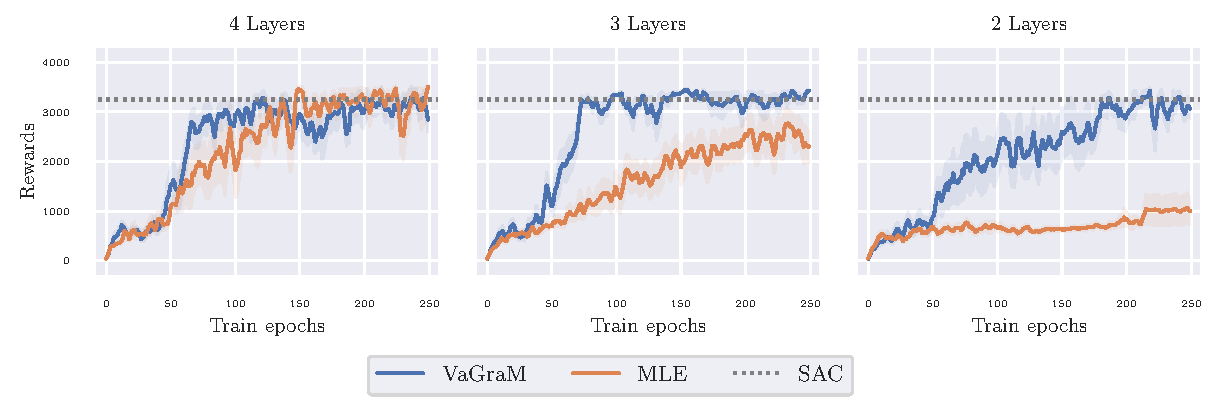
\includegraphics[clip, trim=0.2cm 0.0cm 0.4cm 0.0cm, width=1.\linewidth]{figures/vagram/fig_2.pdf}
\end{center}
    \caption{\textbf{Performance of VaGraM and MLE models with reduced model size}. The dotted lines correspond to the final performance reported for model-free SAC (grey, approx. 3200). Shaded area represents standard error over 16 repeated runs. VaGraM continues to solve the task almost unimpeded, while MLE is unable to even stabilize the Hopper when using a two layer neural network.}
    \label{fig:vagram:pendulum_small}
\end{figure}
Due to the limited complexity of the pendulum environment, the quantitative differences between the mean squared error and VaGraM are at times insignificant in this setting.
The dynamics function of the environment can be approximated sufficiently well with a simple neural network and one hidden layer.

The underlying theory supporting VAML states that a value-aware loss is preferable to a mean squared error loss in a setting where the capacity of the model is too small to fully approximate the problem or the state space contains dimensions that are irrelevant for the control problem.
To test whether our loss function is superior to a maximum likelihood approach in these cases, we used the Hopper environment from the OpenAI gym benchmark \parencite{brockman2016openai}. 
As a deep learning based Dyna algorithm, we chose \ac{mbpo} \parencite{mbpo} and ran all of our experiments using the implementation provided by \cite{pineda2021mbrl}.
We kept the structure of the \ac{mbpo} algorithm and models and replaced the model loss function with VaGraM.

\subsection{Hopper with reduced model capacity}
In the first experiment, we decreased the network size of the used neural network ensemble.
\cite{mbpo} use fully connected neural networks with four hidden layers and 200 neurons per layer.
To test the performance of the algorithm under smaller models, we ran tests with two and three layer networks and 64 neurons per hidden layer.
The results are shown in \autoref{fig:vagram:pendulum_small}.
As before, when using a sufficiently powerful function approximation, we see no difference between the maximum likelihood approach and VaGraM, suggesting that the networks are flexible enough to capture the true environment's dynamics sufficiently close for planning.
But when reducing the model size, the maximum likelihood models quickly lose performance, completely failing to even stabilize the Hopper for a short period in the smallest setting, while VaGraM retains almost its original performance.

\subsection{Hopper with distracting dimensions}


\begin{figure}[t]
    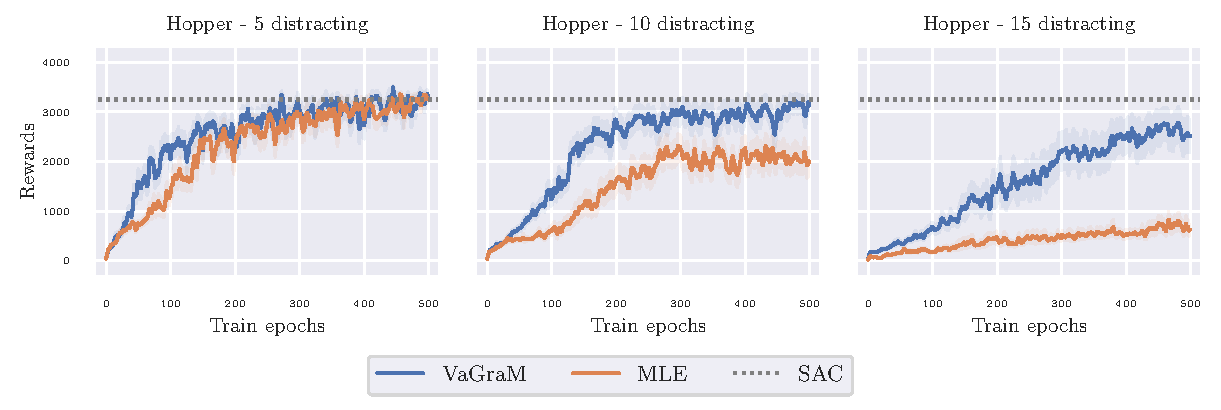
\includegraphics[clip, trim=0.2cm 0.0cm 0.4cm 0.0cm, width=1.\linewidth]{figures/vagram/fig_1.pdf}
    \caption{\textbf{Performance of VaGraM and MLE models with distracting state dimensions}. The dotted lines correspond to the final performance achieved by both algorithms on the Hopper task without distraction (grey, approx. 3200). Shaded area represents standard error over 16 repeated runs. VaGraM achieves significantly higher returns than the MLE baseline, especially in the most challenging setting with 15 distracting dimensions.}
    \label{fig:vagram:pendulum_distraction}
\end{figure}

To show that VaGraM is able to achieve good performance in a setting where there are additional dynamics in the environment that do not contribute to the control problem, we appended distracting dimensions to the Hopper observations.
This mirrors the experimental setup used in \autoref{chap:understanding}.
These are independent of the original environment state space and reward function, and evolve under non-linear and discontinuous dynamics (details in \autoref{app:vagram:implementation}).
A setting with distracting dimensions is known to pose difficulty for model-based control algorithms \parencite{stone2021thedc} and neural networks struggle to model non-linear, discontinuous dynamics, so with an increasing number of dimensions the task becomes harder.

The results of this experiment are shown in \autoref{fig:vagram:pendulum_distraction}.
When using five distracting dimensions, both models are able to capture the dynamics sufficiently well to achieve comparable reward to the original environment.
When increasing the number of dimensions, the performance of the MLE model deteriorates, as more and more of its capacity is used to model the added dynamics.
VaGraM continues to be able to achieve reward even under the presence of distracting dimensions, since the gradient of the value function with regards to the state dimensions which are irrelevant to the control problem becomes small over training.
Still, the performance of VaGraM also suffers with increasing dimensions: when adding 20 distracting dimensions, neither algorithm is able to stabilize the Hopper consistently.
In this case, the value function approximation cannot differentiate sufficiently between the relevant and irrelevant dimensions with the amount of environment samples provided.
%This loss in performance is documented in the literature for model-free reinforcement learning as well and mitigating it is an active area of research \parencite{Stone2021TheDC}.

In summary, we find that VaGraM is able to deal with challenging distractions and reduced model capacity significantly better than a MLE baseline. This validates that our algorithm is really value-aware and can use the value function information \revised{to improve the performance of a model-based controller in settings where the model is unable to fully represent the environment.}

\section{Related work}

Several authors have noted on the problem of learning models that align with the goal of obtaining a good policy. The proposed approaches fall into three broad categories: value-function or policy dependency, representation learning, and data resampling.

Inspired by VAML, \cite{abachi2020policy} present a method that seeks to align the policy gradients under a learned model with the gradients under the true environment. Similar to our proposal, \cite{doro2020gradient} also proposed to reweigh samples in a log likelihood loss, but used policy search as the reinforcement learning approach and did not account for individual state dimensions. \cite{nikishin2021control} show an approach to directly optimizing the policy performance on the real environment by learning a model with implicit differentiation. \cite{asadi2018equivalence} show that the original VAML loss coincides with a Wasserstein distance in the model space under the assumption that the value function is Lipschitz smooth. We find that all of these approaches suffer from similar scaling issues as VAML and have not been shown to lead to strong empirical performance outside of toy settings.

\cite{grimm2020value} characterize the space of possible solutions to the model learning problem under different restrictions given by value functions and policies, and propose to learn models that are value-equivalent, similar to \cite{vaml}. In a follow-up work \cite{grimm2021proper} expand on this idea and show that their principle can be used to improve the MuZero algorithm \parencite{schrittwieser2020mastering}. However, these works do not discuss the optimization challenges in actually finding such value-equivalent models, they mostly characterize the space under different value functions and policies, and present an orthogonal research direction to this chapter.

An alternative to characterizing the problem in the state space of the MDP are representation learning approaches, which seek to map the original states to a latent representation that is more amenable to control. Such approaches include Value Prediction Networks \parencite{oh2017value}, Embed-to-Control \parencite{10.5555/2969442.2969546} and related proposals \parencite{levine2020prediction,cui2021controlaware}. \cite{zhang2021learning} build on the idea of bisimulation metrics \parencite{ferns2004metrics,ferns2011bisimulation} which seeks to characterize the difference between MDPs by finding a state mapping that is reward-invariant under policy and value function. 
In this work, we did not investigate learning state embeddings, but combining our work with representation learning approaches is an exciting direction for future research.

\cite{lambert202objective} hypothesize that the objective mismatch could be solved by reweighing the training buffer for model learning to prioritize data points with high value. These are more likely to matter for obtaining an optimal policy. A similar proposal was evaluated empirically by \cite{nair2020goal}. Contrary to our work however, this technique cannot account for the differing impact of the state space dimensions and scaling, since the data points are weighted as a whole.


\section{Conclusion}
This chapter presents a core issue with using decision-aware methods such as VAML and IterVAML.
It shows that prior work does not account for two important optimization phenomena that appear when learning models with empirical value function approximations.
To mitigate this issue, we introduced an attempt at getting the best of both decision-aware and general purpose learning, Value-Gradient Weighted Model Learning (VaGraM).
VaGraM is a novel loss function to train models that model a dynamics function \emph{where it matters} for the control problem.
We highlighted how VaGraM counters the issues of pure decision-aware learning and show the increased stability of the training procedure when using our loss in a pedagogical environment.

On the Mujoco benchmark, VaGraM performs on par with maximum likelihood estimation when using large neural network models.
However, introducing additional complications to the problem results in drastic performance impacts for MLE based models, which highlights the necessity for value function aware losses in challenging environments and settings in which sufficient model capacity cannot be guaranteed.
In these cases, value-awareness can greatly increase the performance of Dyna algorithms by focusing the model learning procedure on relevant aspects of the state space.
In future work we seek to scale our loss function to image-based RL, where relevant state space dimensions can vary over a task due to shifting camera angles. 
Furthermore, we seek to derive a related value-aware approach for partially observable domains that can take the state inference problem into account.

While VaGraM is an important step towards our goal of unifying general purpose and decision-aware learning, it does not take into account the importance of feature learning.
Therefore we will take a closer look at representations that emerge from latent models in the next chapter.